\begin{figure*}[t]
\centering
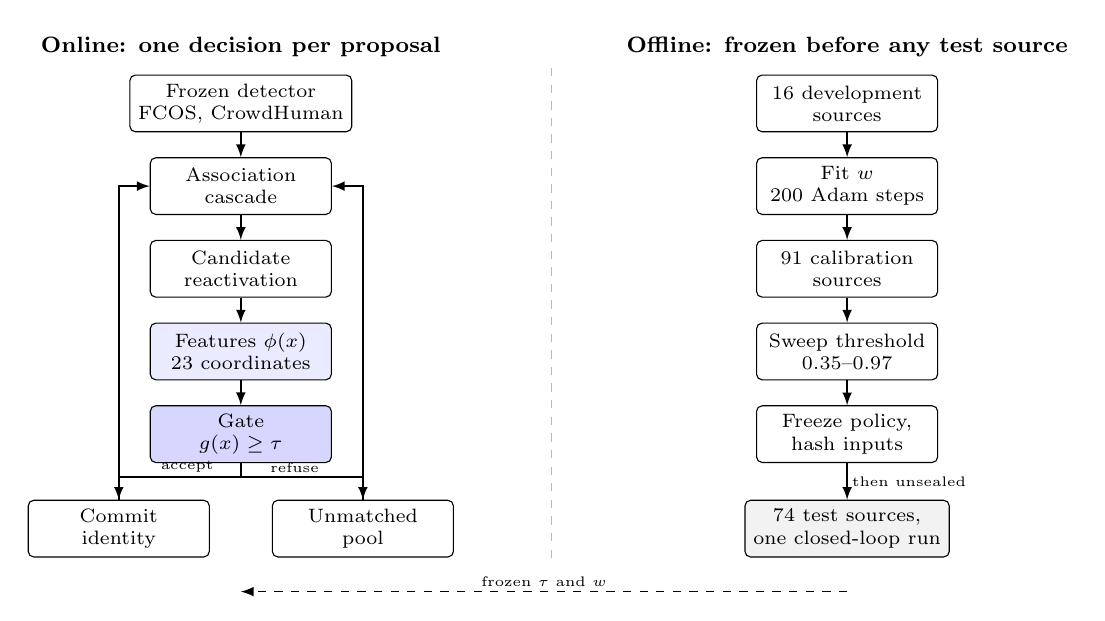
\begin{tikzpicture}[
  box/.style={draw, rounded corners=2pt, align=center, font=\scriptsize,
              inner sep=3pt, minimum height=7.2mm, minimum width=23mm},
  arr/.style={-latex, semithick},
  lbl/.style={font=\tiny, inner sep=1.5pt},
  panel/.style={font=\footnotesize\bfseries}
]

% ---------- panel titles ----------
\node[panel] at (2.40, 0.72) {Online: one decision per proposal};
\node[panel] at (10.10, 0.72) {Offline: frozen before any test source};
\draw[dashed, gray!55] (6.35, 0.45) -- (6.35, -5.85);

% ---------- left: the online loop ----------
\node[box] (det)    at (2.40,  0.00) {Frozen detector\\FCOS, CrowdHuman};
\node[box] (casc)   at (2.40, -1.05) {Association\\cascade};
\node[box] (prop)   at (2.40, -2.10) {Candidate\\reactivation};
\node[box, fill=blue!8]  (feat) at (2.40, -3.15) {Features $\phi(x)$\\23 coordinates};
\node[box, fill=blue!16] (gate) at (2.40, -4.20) {Gate\\$g(x)\geq\tau$};
\node[box] (commit) at (0.85, -5.40) {Commit\\identity};
\node[box] (pool)   at (3.95, -5.40) {Unmatched\\pool};

\draw[arr] (det) -- (casc);
\draw[arr] (casc) -- (prop);
\draw[arr] (prop) -- (feat);
\draw[arr] (feat) -- (gate);
\draw[arr] (gate.south) -- ++(0,-0.18) -| node[lbl, above, pos=0.22] {accept} (commit.north);
\draw[arr] (gate.south) -- ++(0,-0.18) -| node[lbl, above, pos=0.22] {refuse} (pool.north);

% both outcomes return to the cascade at the next step
\draw[arr] (commit.north) -- ++(0,0.30) |- (casc.west);
\draw[arr] (pool.north)   -- ++(0,0.30) |- (casc.east);

% ---------- right: the offline protocol ----------
\node[box] (dev)   at (10.10,  0.00) {16 development\\sources};
\node[box] (fit)   at (10.10, -1.05) {Fit $w$\\200 Adam steps};
\node[box] (cal)   at (10.10, -2.10) {91 calibration\\sources};
\node[box] (sweep) at (10.10, -3.15) {Sweep threshold\\$0.35$--$0.97$};
\node[box] (lock)  at (10.10, -4.20) {Freeze policy,\\hash inputs};
\node[box, fill=gray!10] (test) at (10.10, -5.40) {74 test sources,\\one closed-loop run};

\draw[arr] (dev) -- (fit);
\draw[arr] (fit) -- (cal);
\draw[arr] (cal) -- (sweep);
\draw[arr] (sweep) -- (lock);
\draw[arr] (lock) -- node[lbl, right, pos=0.5] {then unsealed} (test);

% ---------- what the offline column hands to the online one ----------
\draw[arr, dashed] (10.10,-6.20) -- node[lbl, above] {frozen $\tau$ and $w$} (2.40,-6.20);

\end{tikzpicture}
\caption{The method end to end. The left loop runs once per candidate
reactivation at run time: the association cascade proposes a return, the
gate scores it from the 23 coordinates of Section~3, and the outcome either
commits the identity or returns the detection to the unmatched pool, where
the next association step meets it again. The right column is what has to be
settled before the loop may run on a test source: weights are fit on
development sources, the threshold is chosen on calibration sources, and
then the policy is frozen and hashed. Both sides read the same feature
definition, which is what makes a frozen threshold mean anything.}
\label{fig:framework}
\end{figure*}
